\documentclass{article}
\usepackage[utf8]{inputenc}
\usepackage{amsmath}
\usepackage{graphicx}
\usepackage{float}
\usepackage{subcaption}
\usepackage[style=ieee, backend=biber ,citestyle=numeric-comp]{biblatex}
\usepackage{indentfirst}
\usepackage{chngcntr}
\usepackage[a4paper]{geometry}
\usepackage{fancyhdr}
\usepackage[hidelinks]{hyperref}
\usepackage{mathrsfs}
\usepackage[toc,page]{appendix}
\usepackage[longtable]{multirow}
\usepackage{longtable}
\usepackage{booktabs} % Para tablas súper pro
\usepackage{vcell}
\usepackage{array}
\usepackage{epsfig}
\usepackage{pdfpages}
\usepackage{amssymb}
\usepackage{pmboxdraw}
\usepackage{alltt}
\usepackage{listings}
\usepackage{listingsutf8}
\usepackage[english]{babel} % Para que ponga tabla en vez de cuadro
\usepackage{xcolor}
\usepackage{url}
\addbibresource{bibliography.bib}

\usepackage{cancel} % Para tachar términos de ecuaciones
\usepackage{siunitx}




\lstset{
     literate=%
         {á}{{\'a}}1
         {í}{{\'i}}1
         {é}{{\'e}}1
         {ú}{{\'u}}1
         {ó}{{\'o}}1
         {Á}{{\'A}}1
         {Í}{{\'I}}1
         {É}{{\'E}}1
         {Ú}{{\'U}}1
         {Ó}{{\'O}}1}

\definecolor{codegreen}{rgb}{0,0.6,0}
\definecolor{codegray}{rgb}{0.5,0.5,0.5}
\definecolor{codepurple}{rgb}{0.58,0,0.82}
\definecolor{backcolour}{rgb}{0.95,0.95,0.92}

\lstdefinestyle{mystyle}{
    backgroundcolor=\color{backcolour},   
    commentstyle=\color{codegreen},
    keywordstyle=\color{magenta},
    numberstyle=\tiny\color{codegray},
    stringstyle=\color{codepurple},
    basicstyle=\ttfamily\footnotesize,
    breakatwhitespace=false,         
    breaklines=true,                 
    captionpos=b,                    
    keepspaces=true,                 
    numbers=left,                    
    numbersep=5pt,                  
    showspaces=false,                
    showstringspaces=false,
    showtabs=false,                  
    tabsize=2
}
\lstset{style=mystyle}


\numberwithin{equation}{section}
\numberwithin{equation}{subsection}
\counterwithin{figure}{section}
\counterwithin{table}{section}
\AtBeginDocument{\counterwithin{lstlisting}{section}}

%\renewcommand{\tablename}{Tabla}
%\renewcommand{\spanishtablename}{Tabla}
%\renewcommand{\figurename}{Figura}
%\renewcommand{\contentsname}{Contenidos}
%\renewcommand{\listfigurename}{Lista de figuras}
%\renewcommand{\listtablename}{Lista de tablas}
%\renewcommand{\lstlistingname}{Algoritmo}
%\renewcommand{\figureautorefname}{Figura}
%\renewcommand{\tableautorefname}{Tabla}
%\renewcommand{\equationautorefname}{Ecuación}
%\renewcommand{\sectionautorefname}{Sección}
%\renewcommand{\subsectionautorefname}{Apartado}
% \renewcommand{\thesection}{Sección \Arabic{section}}


\geometry{top=3.5cm, bottom=3.5cm, left=3cm, right=3cm}

\pagestyle{fancy}
\fancyhf{}
\lhead{High-frequency vibroacoustic analysis}
\rhead{
\includegraphics[height=0.8cm]{logomuse2}} % right logo
\cfoot{\thepage}



\begin{document}

\begin{center}
\thispagestyle{empty}


\includegraphics[width=16.5cm]{Logo_portada.png} \\

\vspace{2.5cm}

{\huge \textbf{Polytechnic University of Madrid}}\\
\vspace{1cm} 
{\scshape\Large Structures for Space Use \par}
\begin{center}
\vspace{3.5 cm}
{\bfseries\Huge High-frequency vibroacoustic analysis of a structural model. \par}
\vspace{7 cm}

\vfill
{\Large Author:  \par}
{\Large Inés Arauzo Andrés \par}

\end{center}
\end{center}

\pagenumbering{gobble}
\thispagestyle{empty}

\newpage
\pagenumbering{Roman} % Numeración romana hasta la primera sección


\tableofcontents

\newpage
\listoffigures

%\newpage
%\listoftables


\setlength{\parskip}{4mm}
\setlength{\parindent}{20pt}
\setlength{\headheight}{16.07225pt}

\newpage
\pagenumbering{arabic}


\input{Secciones/1 Introducción.tex}
\section{Statement} \label{sec: stat}

The statement of the curret project can be found in \cite{enunciado}. The aim is to define the structural behavior of a determined asrospace structure, that is modelled by three aluminum thin panels ($L_1=1.25$ m,$L_2=1$ m and $t=5\cdot 10^{-3}$ m, see \autoref{fig: enunciado}) with a separation $t = 5\cdot 10^{-2}$ between them, forming two air layers. The properties of the panels are defined on \autoref{tab: panel} whereas the air layer's ones  can be seen on \autoref{tab: air}.


\begin{figure}[htpb]
 \centering
    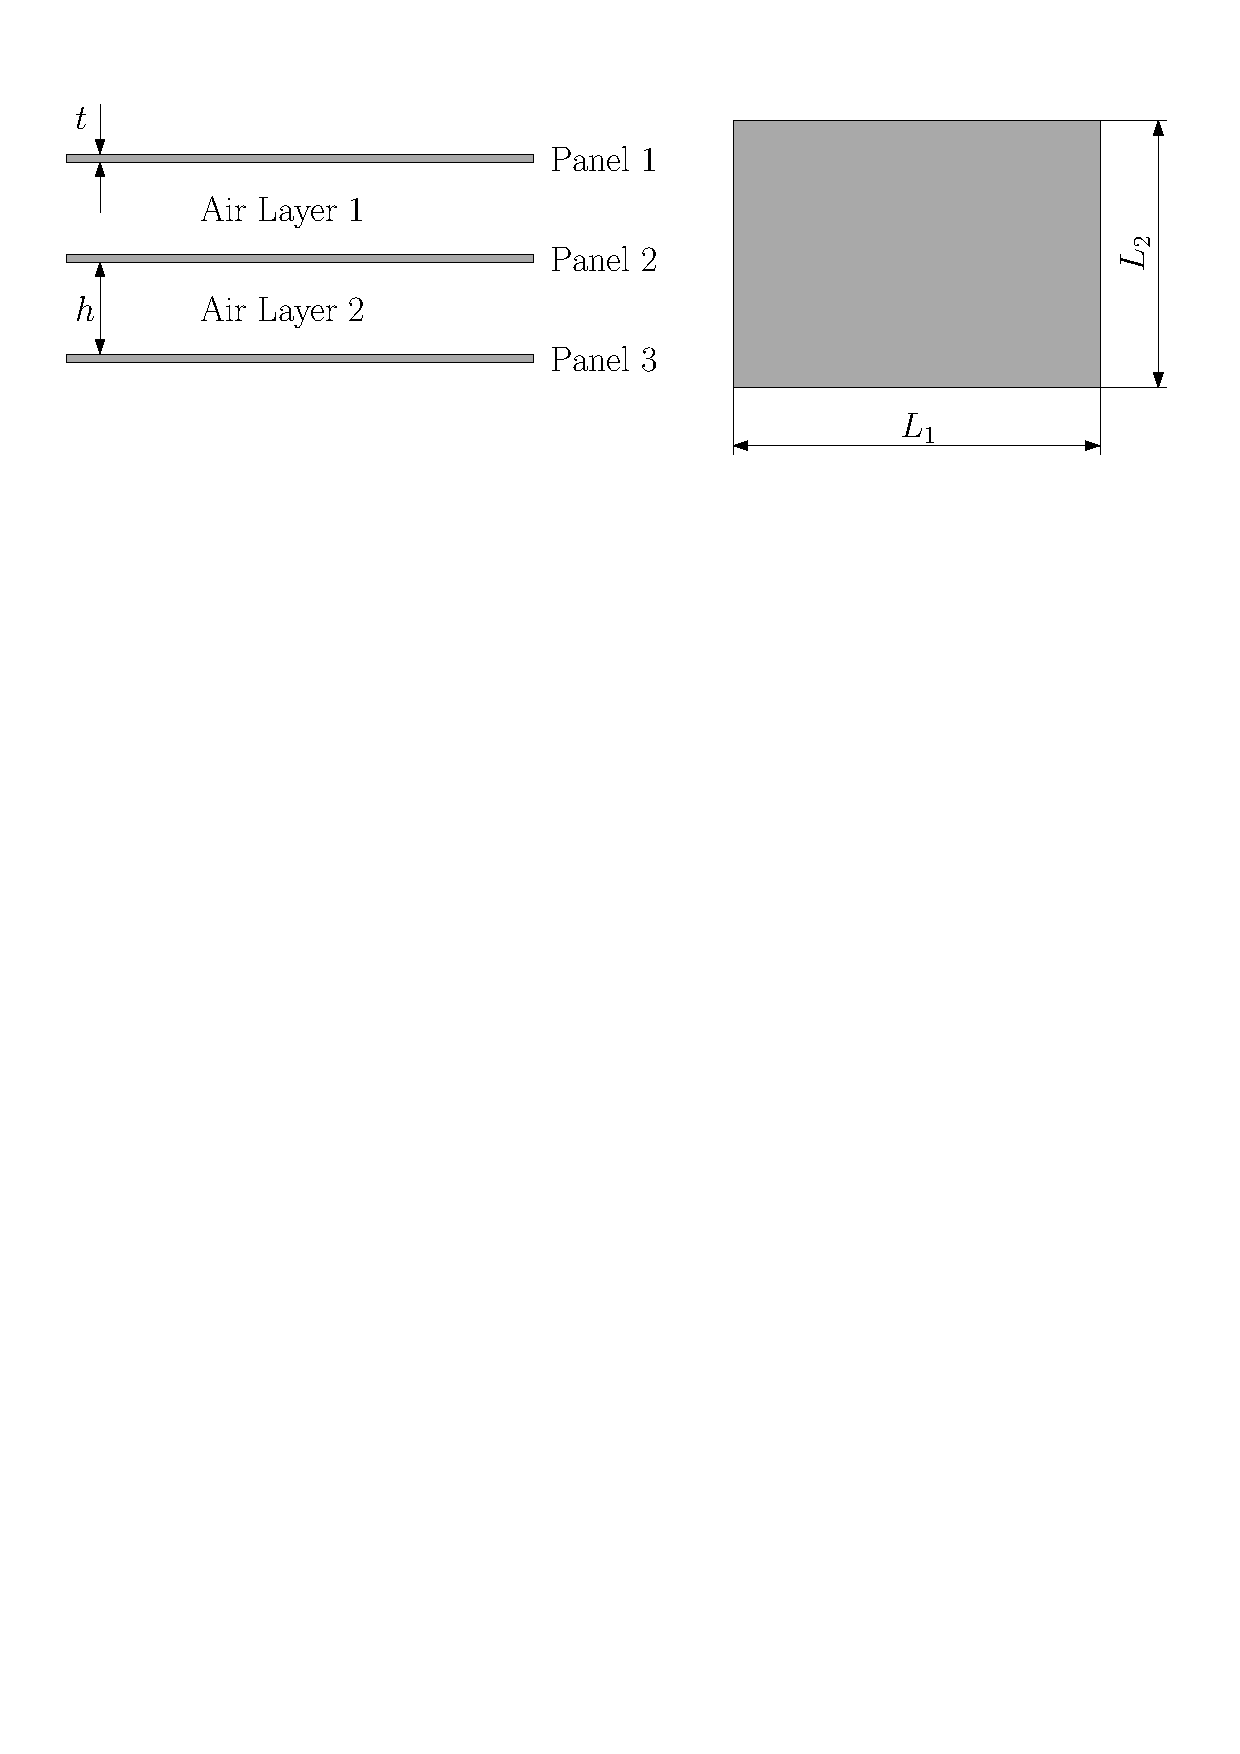
\includegraphics[scale=0.75]{Figures/enunciado.pdf}
  \caption{System of analysis.}
  \label{fig: enunciado}
\end{figure}

\begin{table}[h]
    \caption{Panel properties.}
    \label{tab: panel}
    \centering
    \begin{tabular}{ccc}
    \toprule 
        $\boldsymbol{\rho} 		[\frac{\text{kg}}{\text{m}^3}]$  & $\boldsymbol{E} [\text{Pa}]$ &$\boldsymbol{\nu}[-]$ \\
        2700 & $70\cdot 10^{9}$ & 0.33 \\
       
        \bottomrule
    \end{tabular}
\end{table}

\begin{table}[h]
    \caption{Air properties.}
    \label{tab: air}
    \centering
    \begin{tabular}{cc}
    \toprule 
        $\boldsymbol{\rho} 		[\frac{\text{kg}}{\text{m}^3}]$  & $\boldsymbol{c_0} [\frac{\text{m}}{\text{s}}]$  \\
        1.23 & 343 \\
        \bottomrule
    \end{tabular}
\end{table}

The objective is to calculate the average velocity of the panels and the mean quadratic pressure in the air layers at a high- frequency range,  taking into consideration an external excitation on the panels whose distribution is presented in \autoref{tab: potencia}.

\begin{table}[h]
    \caption{Distribution of external power applied on each panel.}
    \label{tab: potencia}
    \centering
    \begin{tabular}{cccc}
    \toprule 
        $\boldsymbol{f} $ \textbf{Hz} &  $\boldsymbol{P_{1}}$ \textbf{[W]} &  $\boldsymbol{P_{2}}$ \textbf{[W]}&  $\boldsymbol{P_{3}}$ \textbf{[W]} \\
        $16 \leq f \leq 1000$ & 10 &  &  \\
        1250 & 20 & 8.7000 & 20\\
		1600 & 35 & 15.2000 & 35\\ 
		2000 & 50 & 21.7400 & 50\\ 
		2500 & 80 & 36.9600 & 80\\ 
		3150 & 100 & 39.1300 & 100\\ 
		4000 & 150 & 45.6500 & 150\\ 
		$5000 \leq f \leq 10000$ & 100 & 43.4700 & 100\\ 
        \bottomrule
    \end{tabular}
\end{table}

To compute the system response, the following steps must be followed:
\begin{itemize}
\item Calculate the number of modes per bandwidth as a function of frequency for the panels and for the air layers. Specify the frequency from which all the elements of the system can be represented by energetic models, assuming that the high-frequency condition is set at $N \geq 5$ modes.
\item Calculate the cross- coupled dmpling terms ($\eta_pa$ and $\eta_ap$) as a function of frequency.
\item Write down the equations of the SEA model that consist of the 3 panels (only taking into account the bending modes) and the two air layers.
\item Compute and represent the energy  as a function of frequency.
\item Calculate the average speed of the panels and the root mean square pressure of the air as a function of frequency.
\end{itemize}



\newpage
\section{Theoretical foundation} \label{sec: ft}

As previously stated in Section \ref{sec: stat}, the purpose of this study is to obtain the model's response to variable excitation in the high-frequency range. To achieve this, the Statistical Energy Analysis method is employed, which is elucidated in this section.


\subsection{Statistic energy analysis}
Statistical Energy Analysis (SEA) is a method used to analyze the vibrational behavior of complex structures, especially those subjected to high-frequency excitations. The method is based on statistical techniques and assumes that the vibrational energy of a system can be partitioned into discrete energy "bins" that are statistically independent.

To apply the SEA approach, a complex structure is divided into interconnected subsystems, each with its own set of vibrational modes. The energy stored in each subsystem is modeled as a statistical energy distribution, where each mode of vibration behaves as an independent, damped harmonic oscillator. The energy exchange between subsystems is described by coupling coefficients, known as coupling loss factors.

Given the systems $i$ and $j$ (with $i\neq j$) the conservation of the power flux can be applied as,

\begin{align}
P_{i,in} &= P_{i,diss} + P_{ij}\\
P_{j,in} &= P_{j,diss} + P_{ji}
\end{align}

where $P_{i,diss}$ is the internal dissipated power, defined as 
\begin{equation}
P_{i,diss} = \eta_i \omega E_i
\end{equation}
and $P_{ij}$ is the energy exchanged, 
\begin{equation}
P_{ij} = \eta_{ij} \omega E_i -\eta_{ji} \omega E_j
\end{equation}

The combination of these equations result in 

\begin{equation}
P_{i,in} = \eta_i \omega E_i + \omega \sum_{i=0}^N  (\eta_{ij}  E_i -\eta_{ji}  E_j),
\end{equation}

then, knowing that the modal density is 

\begin{equation}
n_i = \frac{N_i}{\Delta \omega},
\end{equation}

there is one last equation derived from the reciprocity relationship between the modal densities:


\begin{equation}
\eta_{ij} n_i = \eta_{ji} n_j
\label{eq: reciproc}
\end{equation}

Applying this process to the analysis system yields the results presented in \autoref{sec: res}.





\newpage
\section{Results} \label{sec: res}

 As stated in \autoref{sec: stat}, the first step to obtain the system's response is to compute the number of modes per bandwidth. The modal density $n_p$ of a thin plate can be expressed as
 \begin{equation}
 n_p(\omega)=\frac{A}{4\pi}\sqrt{\frac{\rho t }{D}}
 \end{equation}
 where $\rho$ is the density, $D$ is the stiffness, $A$ is the area and $t$ the thickness. And being $n_a$ the modal density of the air layers:
 
 \begin{equation}
n_a(\omega)=\frac{V}{\pi c_0} \left(\frac{\omega}{c_0}\right)^2+\frac{A_{air}}{4 c_0}\left(\frac{\omega}{c_0}\right)+\frac{L_{air}}{8 c_0},
\end{equation}  

where $V$ is the volume of the air cavity, $A_{air}$ the area of all the faces defining this volume and $L_{air}$ perimeter defined by it.

Knowing that the number of modes in a bandwidth $\Delta f$ is 
\begin{equation}
N=n\Delta f ,
\end{equation}

the number of modes per bandwidth can be seen in \autoref{fig: modes}, where it can be observed that the high-frequency condition is satisfied at frequencies higher than 315 Hz. Note that this condition is satisffied only when both, the panels and the air layers reach 5 modes per bandwidth.

\begin{figure}[H]
    \centering
    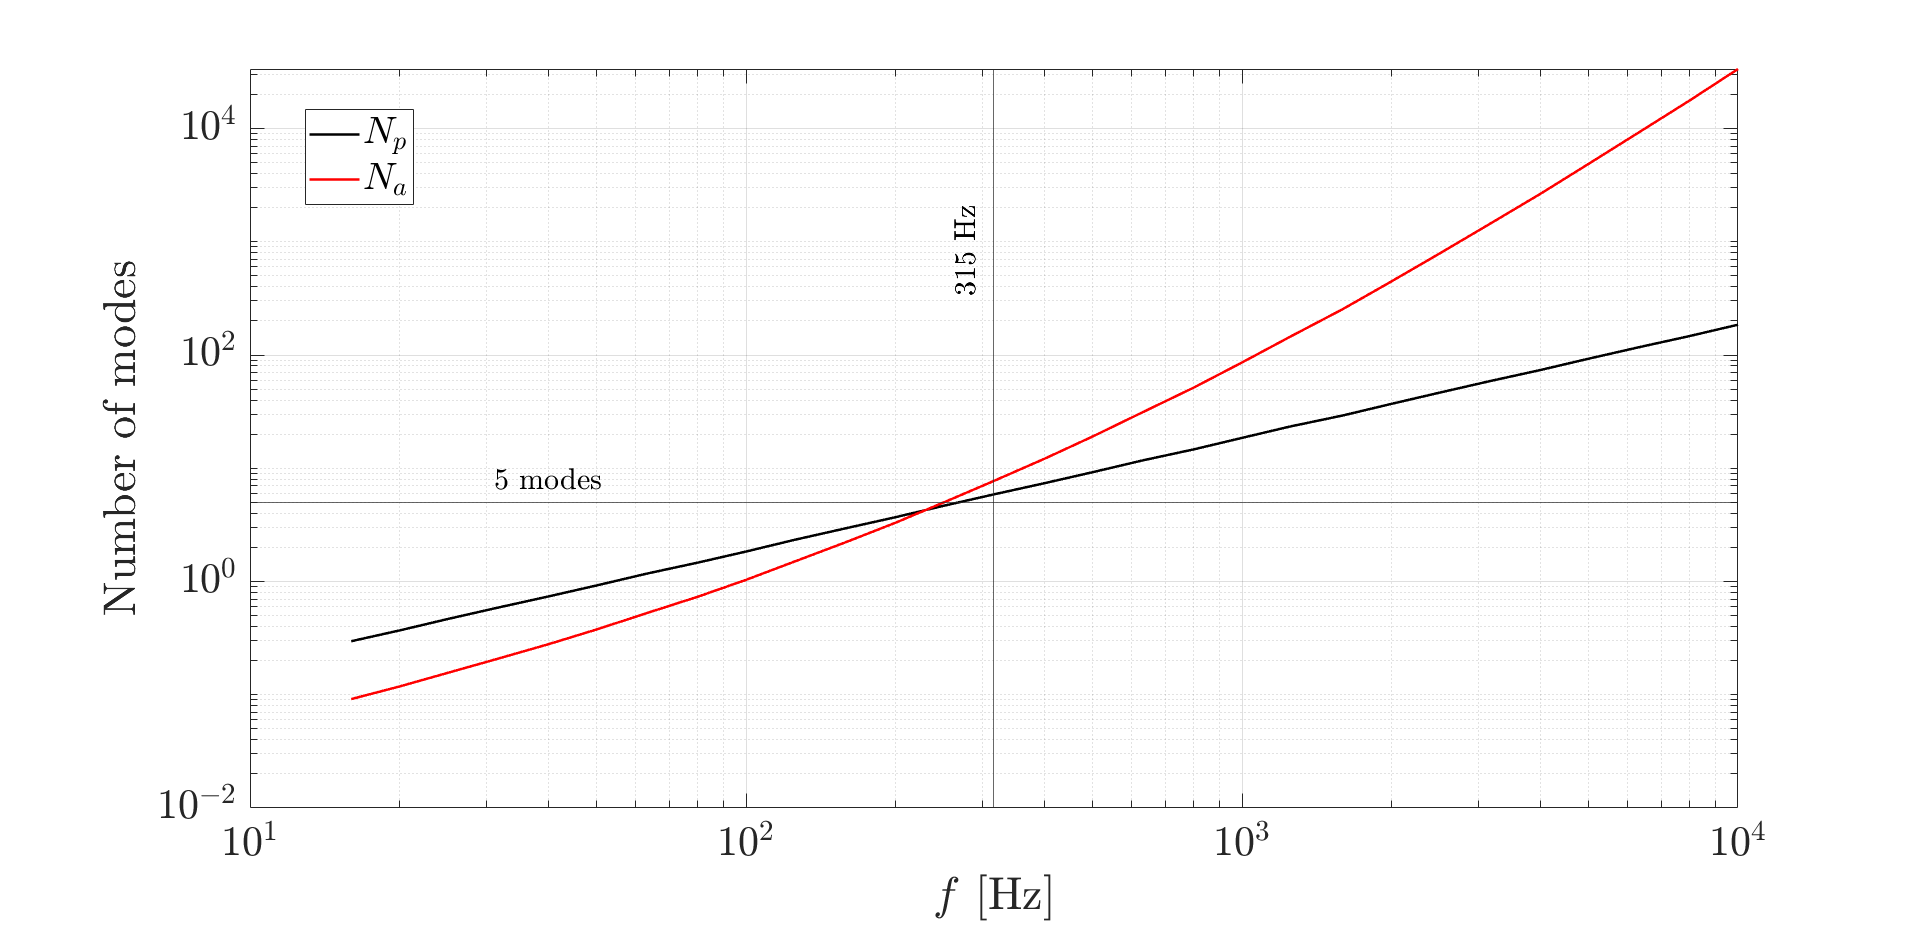
\includegraphics[width=0.75\linewidth]{Figures/modes.png}
    \caption{Number of modes per bandwidth.}
    \label{fig: modes}
\end{figure}

Once the application range of the system is defined, and with the modal densities of the different subsystems calculated, the coupling loss factors (CLF) of the system are defined based on the power radiated by the panels to the air layers, taking into account the radiation efficiency of the panels, as expressed by:

\begin{equation}
\eta_{p a}=\frac{A \rho_0 c_0 \sigma(\omega)}{M \omega},
\end{equation}
where $M$ is the mass of the panel and $\sigma$ is the radiation efficiency of the panel, expressed as
Then, $\eta_{ap}$ is obtained from the reciprocity relation expressed in \autoref{eq: reciproc}. The resulting CLF's are shown in \autoref{fig: etas}

\begin{figure}[H]
    \centering
    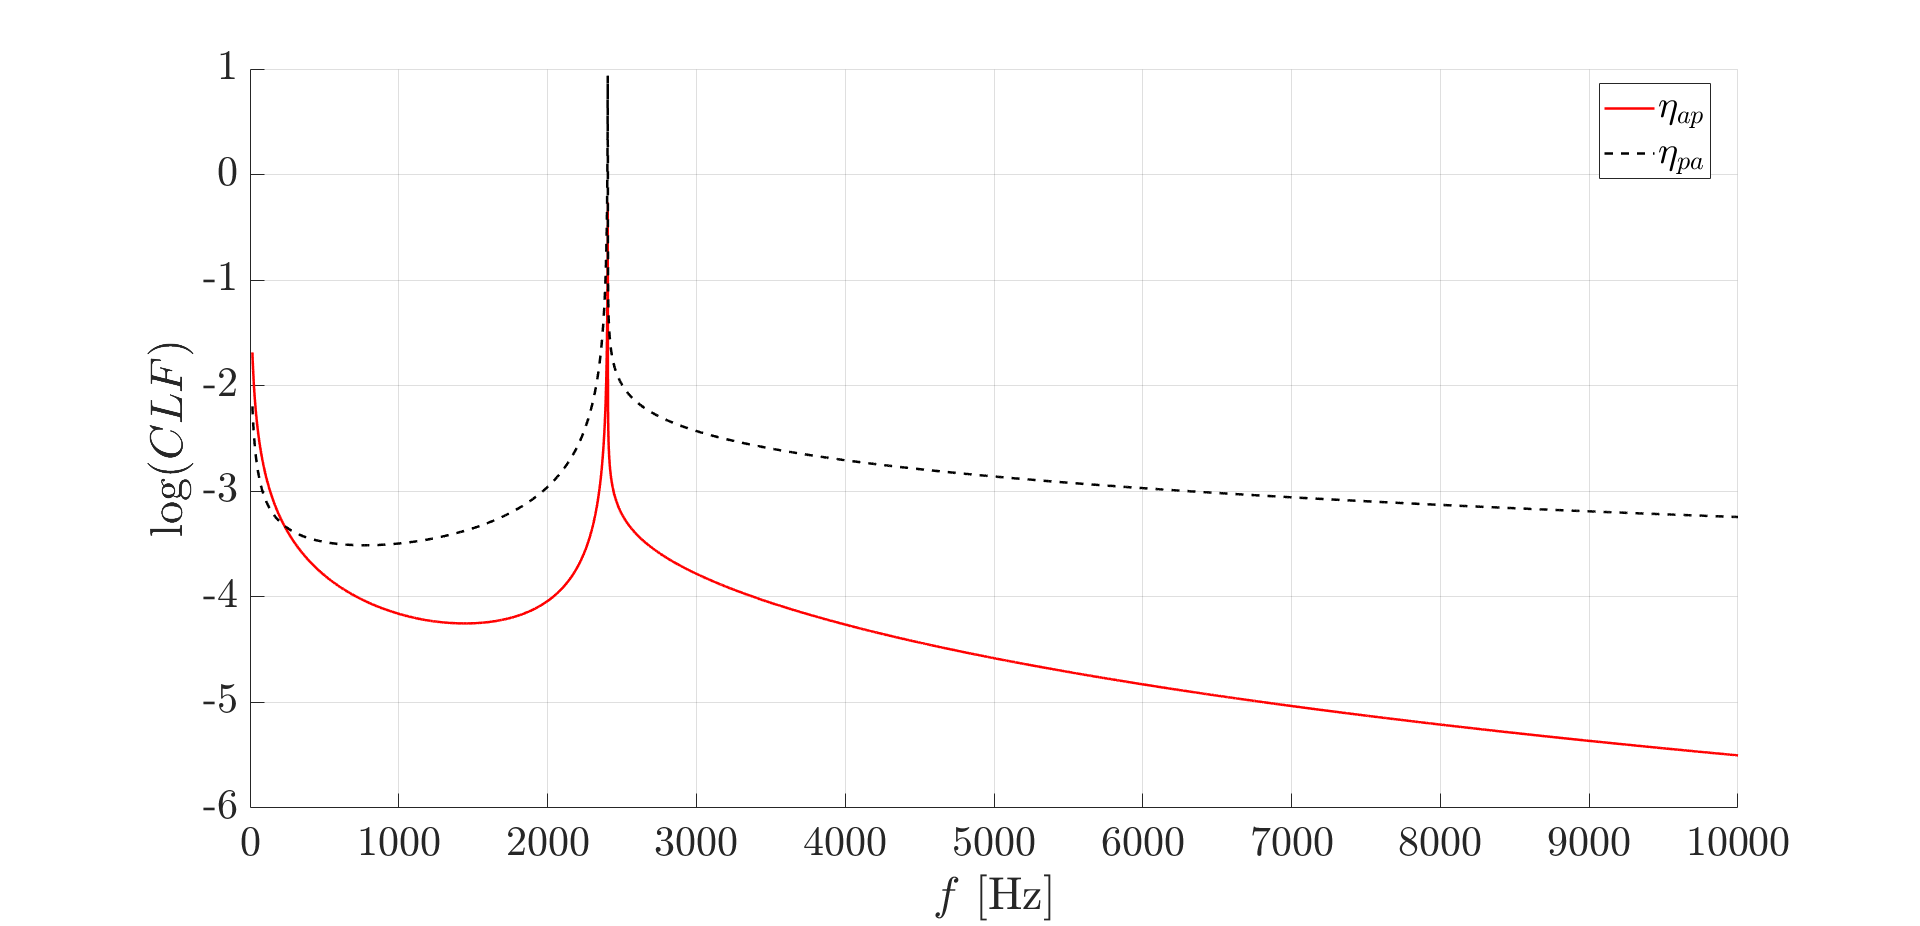
\includegraphics[width=0.75\linewidth]{Figures/etas.png}
    \caption{Coupling loss factors of the panels and the air layers.}
    \label{fig: etas}
\end{figure}

With the CLF's computed, the statistic analysis method can be implemented as shown in \autoref{eq: system}.
\begin{equation}
    \label{eq: system}
    \omega \cdot\left(\begin{array}{ccccc}
    \eta_p+\eta_{p a} & -\eta_{a p} & 0 & 0 & 0 \\
    -\eta_{p a} & \eta_a+\eta_{a p} & -\eta_{p a} & 0 & 0 \\
    0 & -\eta_{a p} & \eta_p+\eta_{p a} & -\eta_{a p} & 0 \\
    0 & 0 & -\eta_{p a} & \eta_a+\eta_{a p} & -\eta_{p a} \\
    0 & 0 & 0 & -\eta_{a p} & \eta_p+\eta_{p a}
    \end{array}\right)\left\{\begin{array}{c}
    E_1 \\
    E_2 \\
    E_3 \\
    E_4 \\
    E_5
    \end{array}\right\}=\left(\begin{array}{c}
    P_1(f) \\
    0 \\
    P_3(f) \\
    0 \\
    P_5(f)
    \end{array}\right)
\end{equation}

Isolating the energies vector in \autoref{eq: system}, the resulting energy of each subsystem can be seen in \autoref{fig: E}

\begin{figure}[H]
    \centering
    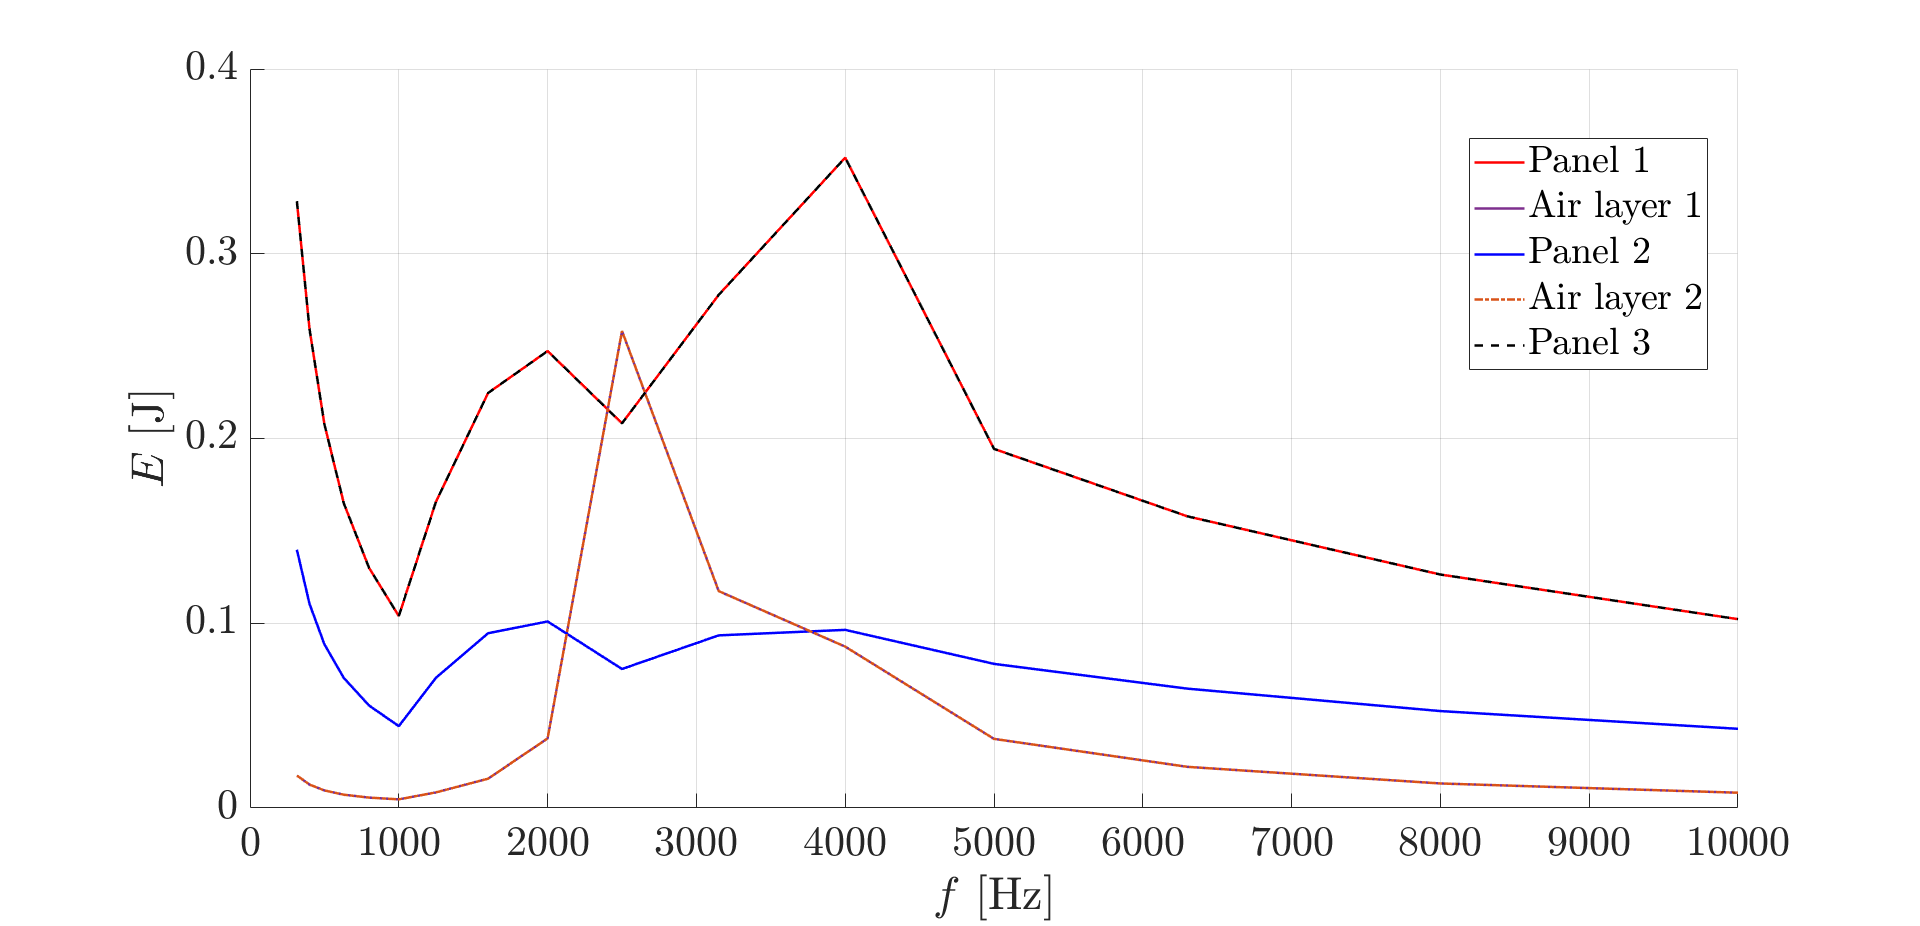
\includegraphics[width=0.75\linewidth]{Figures/E.png}
    \caption{Energy of each subsystem.}
    \label{fig: E}
\end{figure}

Knowing that the energy is related with the average velocity of the panels and with the root mean square pressure of the air  by the following relation,

\begin{equation}
    E = m v^2 = \frac{V}{\rho_0 c_0^2} P^2,
\end{equation}

the response of each subsystem is shown in Figures \ref{fig: pRMS} and \ref{fig: vRMS}
\begin{figure}[H]
    \centering
    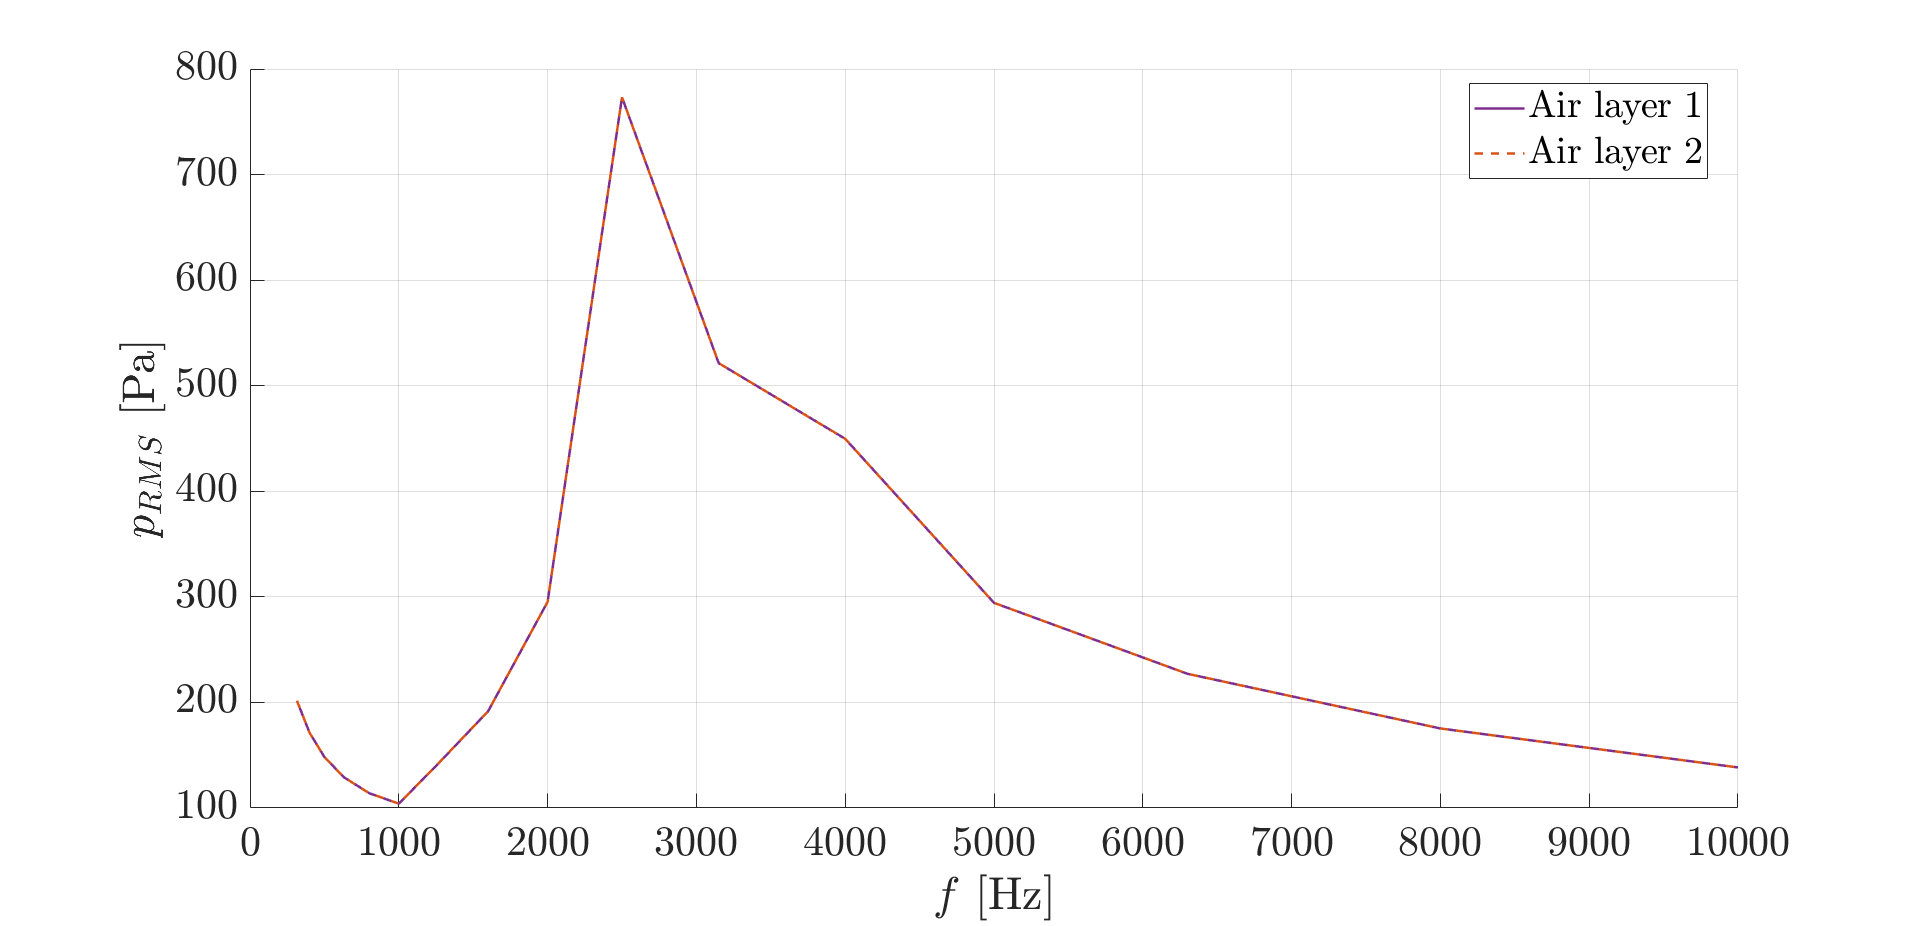
\includegraphics[width=0.75\linewidth]{Figures/pRMS.png}
    \caption{RMS pressure of the air in each air layer.}
    \label{fig: pRMS}
\end{figure}
\begin{figure}[H]
    \centering
    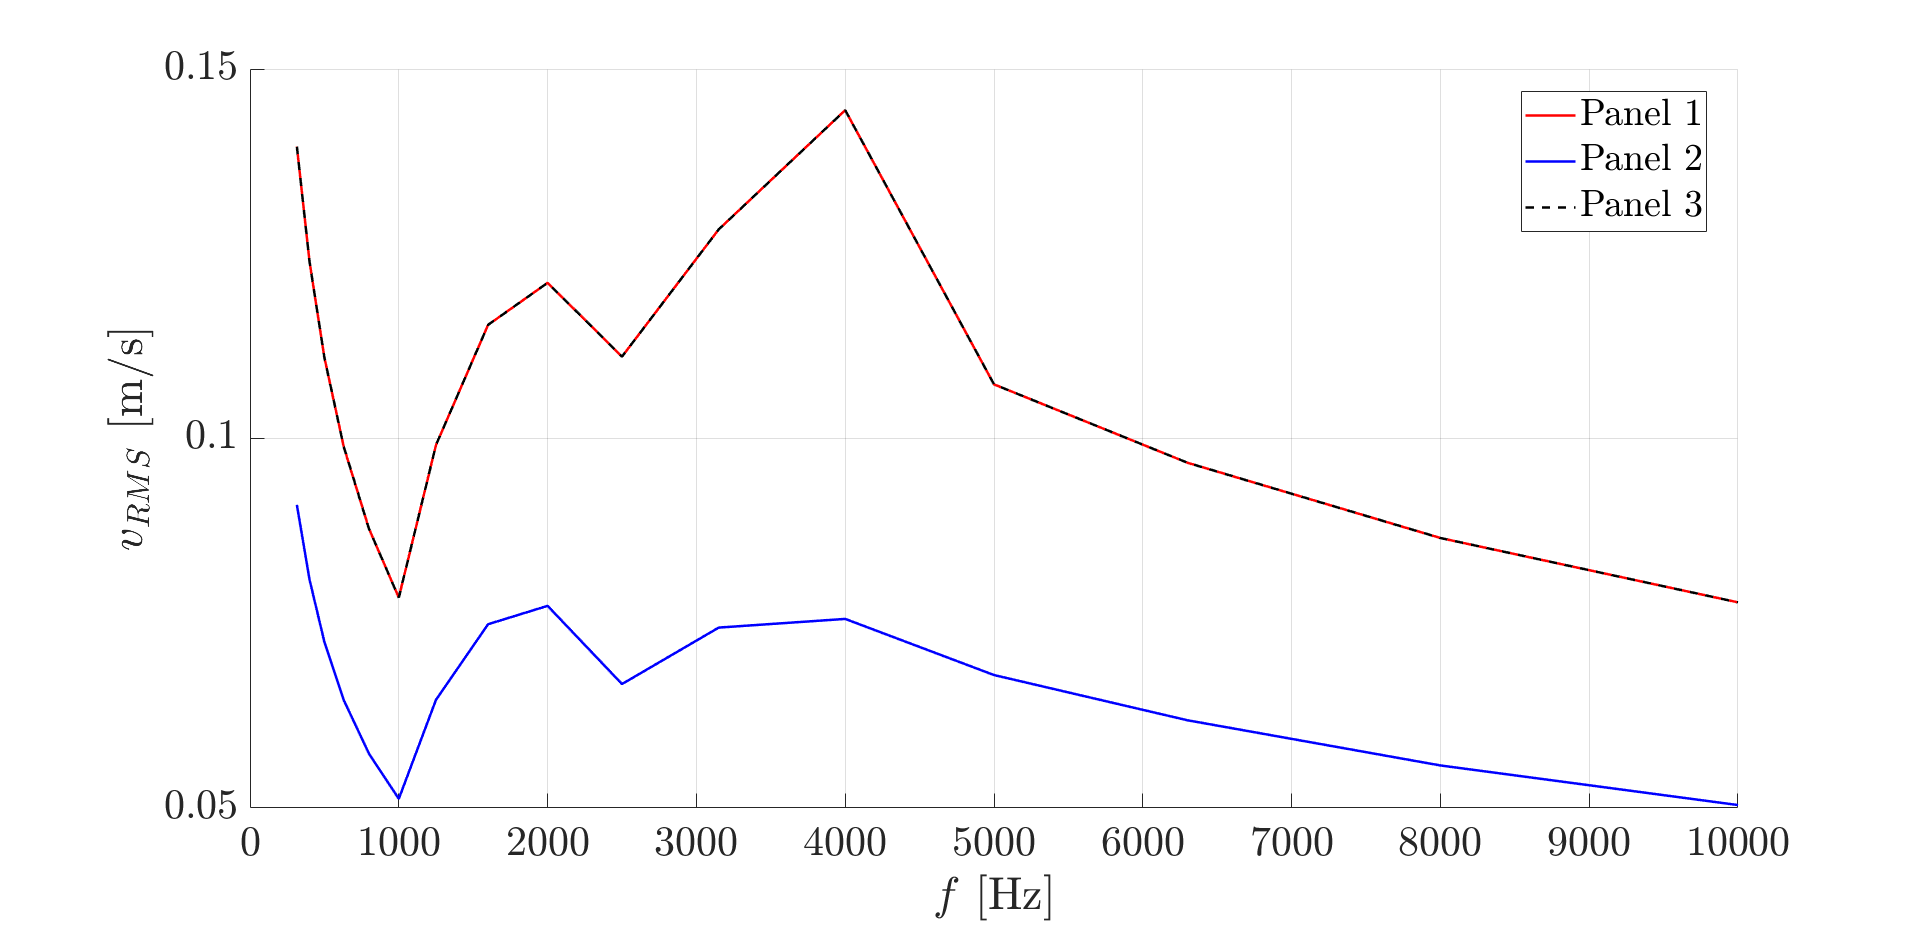
\includegraphics[width=0.75\linewidth]{Figures/vRMS.png}
    \caption{Average velocity of each panel.}
    \label{fig: vRMS}
\end{figure}

Note that as the complete system is symmetric, the responses of the first and third panel, and the responses of the two are layers are exactly the same. Therefore, the central panel's response seems to be damped by the symmetrical response of the rest of subsystems. 

\newpage
\section{Conclusions} \label{sec: conc}
Certain points of interest can be highlighted after the study of the system. 
Firstly, it is important to note the simplicity of the method used in this study. It is truly remarkable that basic algebra and the principle of energy conservation are the only tools necessary to obtain the response of complex systems. This relatively simple example perfectly demonstrates the power of the SEA method for analyzing more complex structures. However, it is important to remember that in this case, the characterization of the different subsystems (obtaining modal densities and CLFs) was given in the problem statement, and the real complexity of this method may come when calculating these values for more complex subsystems.

In conclusion, this project has clarified the concepts taught in the second part of the course regarding vibroacoustics of high-frequency systems.

% \input{Secciones/Resultados.texResultados}
% \input{sECCPropuestas}

%\newpage
%\clearpage


\newpage
\clearpage

\printbibliography[title = {Bibliografía}]

\newpage
\clearpage

% \appendix
% \section{Script de GMAT}

\begin{lstlisting}[language=MATLAB, caption= Scrit de GMAT]

%General Mission Analysis Tool(GMAT) Script
%Created: 2022-11-11 12:56:01


%----------------------------------------
%---------- Spacecraft
%----------------------------------------

Create Spacecraft PequeSpace;
GMAT PequeSpace.DateFormat = UTCGregorian;
GMAT PequeSpace.Epoch = '19 Aug 2014 11:59:28.000';
GMAT PequeSpace.CoordinateSystem = EarthMJ2000Eq;
GMAT PequeSpace.DisplayStateType = Keplerian;
GMAT PequeSpace.SMA = 15738;
GMAT PequeSpace.ECC = 0.5807000000000001;
GMAT PequeSpace.INC = 29.99999999999998;
GMAT PequeSpace.RAAN = 0;
GMAT PequeSpace.AOP = 0;
GMAT PequeSpace.TA = 0;
GMAT PequeSpace.DryMass = 800;
GMAT PequeSpace.Cd = 2.5;
GMAT PequeSpace.Cr = 0;
GMAT PequeSpace.DragArea = 20;
GMAT PequeSpace.SRPArea = 20;
GMAT PequeSpace.SPADDragScaleFactor = 1;
GMAT PequeSpace.SPADSRPScaleFactor = 1;
GMAT PequeSpace.Tanks = {ChemicalTank1};
GMAT PequeSpace.Thrusters = {ChemicalThruster1};
GMAT PequeSpace.NAIFId = -10002001;
GMAT PequeSpace.NAIFIdReferenceFrame = -9002001;
GMAT PequeSpace.OrbitColor = Red;
GMAT PequeSpace.TargetColor = Teal;
GMAT PequeSpace.OrbitErrorCovariance = [ 1e+70 0 0 0 0 0 ; 0 1e+70 0 0 0 0 ; 0 0 1e+70 0 0 0 ; 0 0 0 1e+70 0 0 ; 0 0 0 0 1e+70 0 ; 0 0 0 0 0 1e+70 ];
GMAT PequeSpace.CdSigma = 1e+70;
GMAT PequeSpace.CrSigma = 1e+70;
GMAT PequeSpace.Id = 'SatId';
GMAT PequeSpace.Attitude = CoordinateSystemFixed;
GMAT PequeSpace.SPADSRPInterpolationMethod = Bilinear;
GMAT PequeSpace.SPADSRPScaleFactorSigma = 1e+70;
GMAT PequeSpace.SPADDragInterpolationMethod = Bilinear;
GMAT PequeSpace.SPADDragScaleFactorSigma = 1e+70;
GMAT PequeSpace.ModelFile = 'aura.3ds';
GMAT PequeSpace.ModelOffsetX = 0;
GMAT PequeSpace.ModelOffsetY = 0;
GMAT PequeSpace.ModelOffsetZ = 0;
GMAT PequeSpace.ModelRotationX = 0;
GMAT PequeSpace.ModelRotationY = 0;
GMAT PequeSpace.ModelRotationZ = 0;
GMAT PequeSpace.ModelScale = 1;
GMAT PequeSpace.AttitudeDisplayStateType = 'Quaternion';
GMAT PequeSpace.AttitudeRateDisplayStateType = 'AngularVelocity';
GMAT PequeSpace.AttitudeCoordinateSystem = EarthMJ2000Eq;
GMAT PequeSpace.EulerAngleSequence = '321';



%----------------------------------------
%---------- Spacecraft
%----------------------------------------

Create Spacecraft FalconFoge;
GMAT FalconFoge.DateFormat = UTCGregorian;
GMAT FalconFoge.Epoch = '19 Aug 2014 11:59:28.000';
GMAT FalconFoge.CoordinateSystem = EarthMJ2000Eq;
GMAT FalconFoge.DisplayStateType = Keplerian;
GMAT FalconFoge.SMA = 15738;
GMAT FalconFoge.ECC = 0.5807000000000001;
GMAT FalconFoge.INC = 29.99999999999998;
GMAT FalconFoge.RAAN = 0;
GMAT FalconFoge.AOP = 0;
GMAT FalconFoge.TA = 0;
GMAT FalconFoge.DryMass = 800;
GMAT FalconFoge.Cd = 2.5;
GMAT FalconFoge.Cr = 0;
GMAT FalconFoge.DragArea = 20;
GMAT FalconFoge.SRPArea = 20;
GMAT FalconFoge.SPADDragScaleFactor = 1;
GMAT FalconFoge.SPADSRPScaleFactor = 1;
GMAT FalconFoge.Tanks = {ChemicalTank1};
GMAT FalconFoge.Thrusters = {ChemicalThruster1};
GMAT FalconFoge.NAIFId = -10002001;
GMAT FalconFoge.NAIFIdReferenceFrame = -9002001;
GMAT FalconFoge.OrbitColor = [0 255 0];
GMAT FalconFoge.TargetColor = Teal;
GMAT FalconFoge.OrbitErrorCovariance = [ 1e+70 0 0 0 0 0 ; 0 1e+70 0 0 0 0 ; 0 0 1e+70 0 0 0 ; 0 0 0 1e+70 0 0 ; 0 0 0 0 1e+70 0 ; 0 0 0 0 0 1e+70 ];
GMAT FalconFoge.CdSigma = 1e+70;
GMAT FalconFoge.CrSigma = 1e+70;
GMAT FalconFoge.Id = 'SatId';
GMAT FalconFoge.Attitude = CoordinateSystemFixed;
GMAT FalconFoge.SPADSRPInterpolationMethod = Bilinear;
GMAT FalconFoge.SPADSRPScaleFactorSigma = 1e+70;
GMAT FalconFoge.SPADDragInterpolationMethod = Bilinear;
GMAT FalconFoge.SPADDragScaleFactorSigma = 1e+70;
GMAT FalconFoge.ModelFile = 'aura.3ds';
GMAT FalconFoge.ModelOffsetX = 0;
GMAT FalconFoge.ModelOffsetY = 0;
GMAT FalconFoge.ModelOffsetZ = 0;
GMAT FalconFoge.ModelRotationX = 0;
GMAT FalconFoge.ModelRotationY = 0;
GMAT FalconFoge.ModelRotationZ = 0;
GMAT FalconFoge.ModelScale = 1;
GMAT FalconFoge.AttitudeDisplayStateType = 'Quaternion';
GMAT FalconFoge.AttitudeRateDisplayStateType = 'AngularVelocity';
GMAT FalconFoge.AttitudeCoordinateSystem = EarthMJ2000Eq;
GMAT FalconFoge.EulerAngleSequence = '321';

%----------------------------------------
%---------- Hardware Components
%----------------------------------------

Create ChemicalTank ChemicalTank1;
GMAT ChemicalTank1.AllowNegativeFuelMass = true;
GMAT ChemicalTank1.FuelMass = 20;
GMAT ChemicalTank1.Pressure = 1500;
GMAT ChemicalTank1.Temperature = 20;
GMAT ChemicalTank1.RefTemperature = 20;
GMAT ChemicalTank1.Volume = 0.75;
GMAT ChemicalTank1.FuelDensity = 1260;
GMAT ChemicalTank1.PressureModel = PressureRegulated;

Create ChemicalThruster ChemicalThruster1;
GMAT ChemicalThruster1.CoordinateSystem = Local;
GMAT ChemicalThruster1.Origin = Earth;
GMAT ChemicalThruster1.Axes = VNB;
GMAT ChemicalThruster1.ThrustDirection1 = 1;
GMAT ChemicalThruster1.ThrustDirection2 = 0;
GMAT ChemicalThruster1.ThrustDirection3 = 0;
GMAT ChemicalThruster1.DutyCycle = 1;
GMAT ChemicalThruster1.ThrustScaleFactor = 1;
GMAT ChemicalThruster1.DecrementMass = false;
GMAT ChemicalThruster1.GravitationalAccel = 9.81;
GMAT ChemicalThruster1.C1 = 10;
GMAT ChemicalThruster1.C2 = 0;
GMAT ChemicalThruster1.C3 = 0;
GMAT ChemicalThruster1.C4 = 0;
GMAT ChemicalThruster1.C5 = 0;
GMAT ChemicalThruster1.C6 = 0;
GMAT ChemicalThruster1.C7 = 0;
GMAT ChemicalThruster1.C8 = 0;
GMAT ChemicalThruster1.C9 = 0;
GMAT ChemicalThruster1.C10 = 0;
GMAT ChemicalThruster1.C11 = 0;
GMAT ChemicalThruster1.C12 = 0;
GMAT ChemicalThruster1.C13 = 0;
GMAT ChemicalThruster1.C14 = 0;
GMAT ChemicalThruster1.C15 = 0;
GMAT ChemicalThruster1.C16 = 0;
GMAT ChemicalThruster1.K1 = 300;
GMAT ChemicalThruster1.K2 = 0;
GMAT ChemicalThruster1.K3 = 0;
GMAT ChemicalThruster1.K4 = 0;
GMAT ChemicalThruster1.K5 = 0;
GMAT ChemicalThruster1.K6 = 0;
GMAT ChemicalThruster1.K7 = 0;
GMAT ChemicalThruster1.K8 = 0;
GMAT ChemicalThruster1.K9 = 0;
GMAT ChemicalThruster1.K10 = 0;
GMAT ChemicalThruster1.K11 = 0;
GMAT ChemicalThruster1.K12 = 0;
GMAT ChemicalThruster1.K13 = 0;
GMAT ChemicalThruster1.K14 = 0;
GMAT ChemicalThruster1.K15 = 0;
GMAT ChemicalThruster1.K16 = 0;


%----------------------------------------
%---------- ForceModels
%----------------------------------------

Create ForceModel MarsScape_ForceModel;
GMAT MarsScape_ForceModel.CentralBody = Mars;
GMAT MarsScape_ForceModel.PrimaryBodies = {Mars};
GMAT MarsScape_ForceModel.PointMasses = {Sun};
GMAT MarsScape_ForceModel.Drag = None;
GMAT MarsScape_ForceModel.SRP = Off;
GMAT MarsScape_ForceModel.RelativisticCorrection = Off;
GMAT MarsScape_ForceModel.ErrorControl = RSSStep;
GMAT MarsScape_ForceModel.GravityField.Mars.Degree = 2;
GMAT MarsScape_ForceModel.GravityField.Mars.Order = 0;
GMAT MarsScape_ForceModel.GravityField.Mars.StmLimit = 100;
GMAT MarsScape_ForceModel.GravityField.Mars.PotentialFile = 'Mars50c.cof';
GMAT MarsScape_ForceModel.GravityField.Mars.TideModel = 'None';

Create ForceModel Propagator1_ForceModel;
GMAT Propagator1_ForceModel.CentralBody = Earth;
GMAT Propagator1_ForceModel.PrimaryBodies = {Earth};
GMAT Propagator1_ForceModel.Drag = None;
GMAT Propagator1_ForceModel.SRP = Off;
GMAT Propagator1_ForceModel.RelativisticCorrection = Off;
GMAT Propagator1_ForceModel.ErrorControl = RSSStep;
GMAT Propagator1_ForceModel.GravityField.Earth.Degree = 4;
GMAT Propagator1_ForceModel.GravityField.Earth.Order = 4;
GMAT Propagator1_ForceModel.GravityField.Earth.StmLimit = 100;
GMAT Propagator1_ForceModel.GravityField.Earth.PotentialFile = 'JGM2.cof';
GMAT Propagator1_ForceModel.GravityField.Earth.TideModel = 'None';

Create ForceModel AerobreakingJ2SunProp_ForceModel;
GMAT AerobreakingJ2SunProp_ForceModel.CentralBody = Earth;
GMAT AerobreakingJ2SunProp_ForceModel.PrimaryBodies = {Earth};
GMAT AerobreakingJ2SunProp_ForceModel.PointMasses = {Sun};
GMAT AerobreakingJ2SunProp_ForceModel.SRP = Off;
GMAT AerobreakingJ2SunProp_ForceModel.RelativisticCorrection = Off;
GMAT AerobreakingJ2SunProp_ForceModel.ErrorControl = RSSStep;
GMAT AerobreakingJ2SunProp_ForceModel.GravityField.Earth.Degree = 2;
GMAT AerobreakingJ2SunProp_ForceModel.GravityField.Earth.Order = 0;
GMAT AerobreakingJ2SunProp_ForceModel.GravityField.Earth.StmLimit = 100;
GMAT AerobreakingJ2SunProp_ForceModel.GravityField.Earth.PotentialFile = 'JGM2.cof';
GMAT AerobreakingJ2SunProp_ForceModel.GravityField.Earth.TideModel = 'None';
GMAT AerobreakingJ2SunProp_ForceModel.Drag.AtmosphereModel = JacchiaRoberts;
GMAT AerobreakingJ2SunProp_ForceModel.Drag.HistoricWeatherSource = 'ConstantFluxAndGeoMag';
GMAT AerobreakingJ2SunProp_ForceModel.Drag.PredictedWeatherSource = 'ConstantFluxAndGeoMag';
GMAT AerobreakingJ2SunProp_ForceModel.Drag.CSSISpaceWeatherFile = 'SpaceWeather-All-v1.2.txt';
GMAT AerobreakingJ2SunProp_ForceModel.Drag.SchattenFile = 'SchattenPredict.txt';
GMAT AerobreakingJ2SunProp_ForceModel.Drag.F107 = 150;
GMAT AerobreakingJ2SunProp_ForceModel.Drag.F107A = 150;
GMAT AerobreakingJ2SunProp_ForceModel.Drag.MagneticIndex = 3;
GMAT AerobreakingJ2SunProp_ForceModel.Drag.SchattenErrorModel = 'Nominal';
GMAT AerobreakingJ2SunProp_ForceModel.Drag.SchattenTimingModel = 'NominalCycle';
GMAT AerobreakingJ2SunProp_ForceModel.Drag.DragModel = 'Spherical';

Create ForceModel AerobreakingnoPerturbation_ForceModel;
GMAT AerobreakingnoPerturbation_ForceModel.CentralBody = Earth;
GMAT AerobreakingnoPerturbation_ForceModel.PrimaryBodies = {Earth};
GMAT AerobreakingnoPerturbation_ForceModel.SRP = Off;
GMAT AerobreakingnoPerturbation_ForceModel.RelativisticCorrection = Off;
GMAT AerobreakingnoPerturbation_ForceModel.ErrorControl = RSSStep;
GMAT AerobreakingnoPerturbation_ForceModel.GravityField.Earth.Degree = 1;
GMAT AerobreakingnoPerturbation_ForceModel.GravityField.Earth.Order = 0;
GMAT AerobreakingnoPerturbation_ForceModel.GravityField.Earth.StmLimit = 100;
GMAT AerobreakingnoPerturbation_ForceModel.GravityField.Earth.PotentialFile = 'JGM2.cof';
GMAT AerobreakingnoPerturbation_ForceModel.GravityField.Earth.TideModel = 'None';
GMAT AerobreakingnoPerturbation_ForceModel.Drag.AtmosphereModel = JacchiaRoberts;
GMAT AerobreakingnoPerturbation_ForceModel.Drag.HistoricWeatherSource = 'ConstantFluxAndGeoMag';
GMAT AerobreakingnoPerturbation_ForceModel.Drag.PredictedWeatherSource = 'ConstantFluxAndGeoMag';
GMAT AerobreakingnoPerturbation_ForceModel.Drag.CSSISpaceWeatherFile = 'SpaceWeather-All-v1.2.txt';
GMAT AerobreakingnoPerturbation_ForceModel.Drag.SchattenFile = 'SchattenPredict.txt';
GMAT AerobreakingnoPerturbation_ForceModel.Drag.F107 = 150;
GMAT AerobreakingnoPerturbation_ForceModel.Drag.F107A = 150;
GMAT AerobreakingnoPerturbation_ForceModel.Drag.MagneticIndex = 3;
GMAT AerobreakingnoPerturbation_ForceModel.Drag.SchattenErrorModel = 'Nominal';
GMAT AerobreakingnoPerturbation_ForceModel.Drag.SchattenTimingModel = 'NominalCycle';
GMAT AerobreakingnoPerturbation_ForceModel.Drag.DragModel = 'Spherical';

%----------------------------------------
%---------- Propagators
%----------------------------------------

Create Propagator AerobreakingJ2SunProp;
GMAT AerobreakingJ2SunProp.FM = AerobreakingJ2SunProp_ForceModel;
GMAT AerobreakingJ2SunProp.Type = RungeKutta89;
GMAT AerobreakingJ2SunProp.InitialStepSize = 60;
GMAT AerobreakingJ2SunProp.Accuracy = 9.999999999999999e-12;
GMAT AerobreakingJ2SunProp.MinStep = 0.001;
GMAT AerobreakingJ2SunProp.MaxStep = 2700;
GMAT AerobreakingJ2SunProp.MaxStepAttempts = 50;
GMAT AerobreakingJ2SunProp.StopIfAccuracyIsViolated = true;

Create Propagator AerobreakingnoPerturbation;
GMAT AerobreakingnoPerturbation.FM = AerobreakingnoPerturbation_ForceModel;
GMAT AerobreakingnoPerturbation.Type = RungeKutta89;
GMAT AerobreakingnoPerturbation.InitialStepSize = 60;
GMAT AerobreakingnoPerturbation.Accuracy = 9.999999999999999e-12;
GMAT AerobreakingnoPerturbation.MinStep = 0.001;
GMAT AerobreakingnoPerturbation.MaxStep = 2700;
GMAT AerobreakingnoPerturbation.MaxStepAttempts = 50;
GMAT AerobreakingnoPerturbation.StopIfAccuracyIsViolated = true;

%----------------------------------------
%---------- Coordinate Systems
%----------------------------------------

Create CoordinateSystem MarsInertial;
GMAT MarsInertial.Origin = Mars;
GMAT MarsInertial.Axes = BodyInertial;

%----------------------------------------
%---------- Subscribers
%----------------------------------------

Create OrbitView DefaultOrbitView;
GMAT DefaultOrbitView.SolverIterations = Current;
GMAT DefaultOrbitView.UpperLeft = [ 0.001764705882352941 0.009950248756218905 ];
GMAT DefaultOrbitView.Size = [ 0.5 0.6156716417910447 ];
GMAT DefaultOrbitView.RelativeZOrder = 344;
GMAT DefaultOrbitView.Maximized = false;
GMAT DefaultOrbitView.Add = {PequeSpace, FalconFoge, Earth};
GMAT DefaultOrbitView.CoordinateSystem = EarthMJ2000Eq;
GMAT DefaultOrbitView.DrawObject = [ true true true ];
GMAT DefaultOrbitView.DataCollectFrequency = 1;
GMAT DefaultOrbitView.UpdatePlotFrequency = 50;
GMAT DefaultOrbitView.NumPointsToRedraw = 0;
GMAT DefaultOrbitView.ShowPlot = true;
GMAT DefaultOrbitView.MaxPlotPoints = 20000;
GMAT DefaultOrbitView.ShowLabels = true;
GMAT DefaultOrbitView.ViewPointReference = Earth;
GMAT DefaultOrbitView.ViewPointVector = [ 30000 0 0 ];
GMAT DefaultOrbitView.ViewDirection = Earth;
GMAT DefaultOrbitView.ViewScaleFactor = 1;
GMAT DefaultOrbitView.ViewUpCoordinateSystem = EarthMJ2000Eq;
GMAT DefaultOrbitView.ViewUpAxis = Z;
GMAT DefaultOrbitView.EclipticPlane = Off;
GMAT DefaultOrbitView.XYPlane = On;
GMAT DefaultOrbitView.WireFrame = Off;
GMAT DefaultOrbitView.Axes = On;
GMAT DefaultOrbitView.Grid = Off;
GMAT DefaultOrbitView.SunLine = Off;
GMAT DefaultOrbitView.UseInitialView = On;
GMAT DefaultOrbitView.StarCount = 7000;
GMAT DefaultOrbitView.EnableStars = On;
GMAT DefaultOrbitView.EnableConstellations = On;

Create GroundTrackPlot DefaultGroundTrackPlot;
GMAT DefaultGroundTrackPlot.SolverIterations = Current;
GMAT DefaultGroundTrackPlot.UpperLeft = [ 0 0.4465174129353234 ];
GMAT DefaultGroundTrackPlot.Size = [ 0.5 0.4502487562189055 ];
GMAT DefaultGroundTrackPlot.RelativeZOrder = 176;
GMAT DefaultGroundTrackPlot.Maximized = false;
GMAT DefaultGroundTrackPlot.DataCollectFrequency = 1;
GMAT DefaultGroundTrackPlot.UpdatePlotFrequency = 50;
GMAT DefaultGroundTrackPlot.NumPointsToRedraw = 0;
GMAT DefaultGroundTrackPlot.ShowPlot = true;
GMAT DefaultGroundTrackPlot.MaxPlotPoints = 20000;
GMAT DefaultGroundTrackPlot.CentralBody = Earth;
GMAT DefaultGroundTrackPlot.TextureMap = 'ModifiedBlueMarble.jpg';

Create XYPlot XYPlot1;
GMAT XYPlot1.SolverIterations = Current;
GMAT XYPlot1.UpperLeft = [ 0.5052941176470588 0.008706467661691543 ];
GMAT XYPlot1.Size = [ 0.5 0.4502487562189055 ];
GMAT XYPlot1.RelativeZOrder = 240;
GMAT XYPlot1.Maximized = false;
GMAT XYPlot1.XVariable = PequeSpace.ElapsedDays;
GMAT XYPlot1.YVariables = {PequeSpace.EarthMJ2000Eq.INC};
GMAT XYPlot1.ShowGrid = true;
GMAT XYPlot1.ShowPlot = true;

Create XYPlot XvsRaRp;
GMAT XvsRaRp.SolverIterations = Current;
GMAT XvsRaRp.UpperLeft = [ 0.1788235294117647 0.5149253731343284 ];
GMAT XvsRaRp.Size = [ 0.5 0.4502487562189055 ];
GMAT XvsRaRp.RelativeZOrder = 97;
GMAT XvsRaRp.Maximized = true;
GMAT XvsRaRp.XVariable = PequeSpace.ElapsedDays;
GMAT XvsRaRp.YVariables = {PequeSpace.Earth.RadApo, PequeSpace.Earth.RadPer};
GMAT XvsRaRp.ShowGrid = true;
GMAT XvsRaRp.ShowPlot = true;

Create ReportFile MARTATQ;
GMAT MARTATQ.SolverIterations = Current;
GMAT MARTATQ.UpperLeft = [ 0.1094117647058823 0.150497512437811 ];
GMAT MARTATQ.Size = [ 0.5994117647058823 0.7985074626865671 ];
GMAT MARTATQ.RelativeZOrder = 348;
GMAT MARTATQ.Maximized = false;
GMAT MARTATQ.Filename = 'MARTATEQUEREMOS.txt';
GMAT MARTATQ.Precision = 16;
GMAT MARTATQ.Add = {PequeSpace.Earth.Altitude, PequeSpace.EarthMJ2000Eq.AOP, PequeSpace.Earth.EA, PequeSpace.Earth.ECC, PequeSpace.ElapsedDays, PequeSpace.EarthMJ2000Eq.INC, PequeSpace.Earth.RadApo, PequeSpace.Earth.RadPer, PequeSpace.Earth.SMA, PequeSpace.Earth.TA, FalconFoge.Earth.Altitude, FalconFoge.EarthMJ2000Eq.AOP, FalconFoge.Earth.EA, FalconFoge.Earth.ECC, FalconFoge.EarthMJ2000Eq.INC, FalconFoge.Earth.RadApo, FalconFoge.Earth.RadPer, FalconFoge.Earth.SMA, FalconFoge.Earth.TA};
GMAT MARTATQ.WriteHeaders = true;
GMAT MARTATQ.LeftJustify = On;
GMAT MARTATQ.ZeroFill = Off;
GMAT MARTATQ.FixedWidth = true;
GMAT MARTATQ.Delimiter = ' ';
GMAT MARTATQ.ColumnWidth = 23;
GMAT MARTATQ.WriteReport = true;


%----------------------------------------
%---------- Mission Sequence
%----------------------------------------

BeginMissionSequence;
Propagate Synchronized AerobreakingJ2SunProp(PequeSpace) AerobreakingnoPerturbation(FalconFoge) {FalconFoge.Earth.SMA = 7100, PequeSpace.Earth.ECC = 0.001};


\end{lstlisting}




\end{document}


